\section{Evaluation}
\label{sec:Evaluation}

The team evaluates how they believe the team, the project management and the
finalised project matches up to the project's goals \ref{sec:projectGoals}.

\subsection{Evaluation of the Final Product}

Each of the different modules of the final product are evaluated below: 

\subsubsection{Evaluation of Person and Location Name Detection in Subtitles}
This section evaluates the name and location detection which is performed per subtitle file in the system. This evaluation will be done as described in Section \ref{sec:EvalTechniques} using the follow TV programmes subtitles:
\begin{itemize}
	\item{Doctor Who 2005 Series 2 Episode 13 - Doomsday}
	\item{Top Gear Series 9 Episode 3 - US Special}
\end{itemize}

These two programmes cover different genre types, the use of character and actor names as well as covering both fictional and non fictional names. This enables extensive testing of these detectors. An overview of these episodes is given in Appendix \ref{sec:TV} in sections \ref{sec:TopGearAmerica} and \ref{sec:DrWhoEp13}.

Prior to presenting the results, a few important points need to be made: firstly, the current system doesn’t look to see if the same name is mentioned more than once in the same Subtitle object i.e. a line of speech, otherwise it would lead to repeated sections of the video which was deemed unnecessary. In addition, in order to count where shortened versions of names are used the system has been built to match instances such as ``Amy" with ``Amy Pond" in terms of name count. However this has led to wrong detections being made for example if the word Pond is mentioned it could refer to Amy Pond or Melody Pond and so both of these will count as a mention towards the respective characters.

The tables on the following pages present the results and the time taken to perform manual detection, natural language processing (NLP) for person name and location detection and also, using the list of actors/characters obtained from the Internet Television database.

\newpage
\textbf{\underline{Doctor Who 2005 Series 2 Episode 13 - Doomsday (Duration: 45 minutes)}}

\underline{Manual Person Name Detection}

\begin{center}
\begin{longtable}{|p{160pt}|p{90pt}|p{140pt}|}
\hline
\textbf{Name}					&\textbf{Manual - Count}	&\textbf{Manual - Main Character}	\\\hline
Daleks						&31				&Yes						\\\hline
Cybermen					&30				&Yes						\\\hline
The Doctor					&19				&Yes						\\\hline
Rose Tyler					&19				&Yes						\\\hline
Mickey						&10				&Yes						\\\hline		
Time Lord					&10				&						\\\hline          
Jackie Tyler					&6				&Yes						\\\hline
Pete Tyler						&6				&						\\\hline	          
God							&5				&						\\\hline	          
Mum							&5				&Yes (Refer to Jackie Tyler)	\\\hline
Queen						&4				&						\\\hline		          
The Emperor					&4				&						\\\hline		          
Jacks						&4				&Yes (Refers to Jackie Tyler)	\\\hline
Dad							&4				&						\\\hline		          
Cyberleader One				&3				&						\\\hline		          
Dalek Thay					&2				&						\\\hline		          
Jake							&2				&						\\\hline		          
Stephen Hawking				&1				&						\\\hline		          
Chrissie						&1				&						\\\hline		          
Harriet Jones					&1				&						\\\hline		          
Jacqueline Andrea Suzette Tyler 	&1				& Yes (Refers to Jackie Tyler)	\\\hline
Micketty-Mick-Mickey			&1				& Yes (Refers to Mickey)		\\\hline
Dalek Sec						&1				&						\\\hline		          
DalekJast						&1				&						\\\hline		          
Dalek Caan					&1				&						\\\hline		          
Mutt							&1				&						\\\hline		          
Jeff							&1				&						\\\hline		          
Tylers						&1				&						\\\hline		          
\textbf{Total: 28}				&\textbf{Total: 175}	&						\\\hline		          
\end{longtable}
\end{center}

\newpage
\underline{Manual Location Detection}

\begin{center}
\begin{tabular}{|p{160pt}|p{90pt}|p{140pt}|}
\hline
\textbf{Name}				&\textbf{Manual - Count}		&\textbf{Manual - Main Location}		\\\hline
Genesis Ark			&14					&Yes						\\\hline	
Void					&12					&Yes						\\\hline
Torchwood Institute		&10					&Yes						\\\hline
Hell					&5					&						\\\hline
Planet				&5					&						\\\hline
Earth				&4					&Yes						\\\hline
Country				&4					&						\\\hline
Tardis				&3					&Yes						\\\hline
Sphere Chamber		&3					&						\\\hline
Pete’s World			&2					&						\\\hline
Universe				&2					&						\\\hline
Norway				&2					&						\\\hline
Darlig Ulv Stranden		&2					&						\\\hline		
Staircase				&2					&						\\\hline
Room with the Sphere	&1					&						\\\hline
Parallel Earth			&1					&						\\\hline	
Parallel Torchwood		&1					&						\\\hline
Arcadia				&1					&						\\\hline
Stairwell				&1					&						\\\hline
London				&1					&						\\\hline
Bergen				&1					&						\\\hline
Bad Wolf Bay			&1					&Yes						\\\hline
\textbf{Total: 21}		&\textbf{Total: 64}		&						\\\hline
\end{tabular}
\end{center}

\underline{OpenNLP Person Name Detection}
\begin{center}
\begin{tabular}{|p{160pt}|p{90pt}|p{140pt}|}
\hline
Name						&OpenNLP - Count		&OpenNLP - Main Character\\\hline
Daleks						&31					&Yes				\\\hline
Rose Tyler					&22					&Yes				\\\hline
Doctor						&19					&				\\\hline
Jackie Tyler					&13					&				\\\hline
Pete Tyler						&11					&				\\\hline			
Mr Mickey					&10					&				\\\hline	
Jacqueline Andrea Suzette Tyler	&8					&				\\\hline	
Ah							&6					&				\\\hline	
Lord							&5					&				\\\hline	
Mum 						&5					&				\\\hline	
Sorry						&3					&				\\\hline	
Wait							&2					&				\\\hline	
Stephen Hawking				&1					&				\\\hline	
Harriet Jones					&1					&				\\\hline	
Jeff							&1					&				\\\hline	
\textbf{Total: 21}				&\textbf{Total: 138}		&				\\\hline
\end{tabular}
\end{center}	

\newpage
\underline{OpenNLP Location Name Detection}
\begin{center}
\begin{tabular}{|p{160pt}|p{90pt}|p{140pt}|}
\hline
\textbf{Name}		&\textbf{OpenNLP - Count}	&\textbf{OpenNLP - Main Location}\\\hline
Rose			&19				&Yes		\\\hline
Ark			&14				&		\\\hline
Torchwood	&11				&		\\\hline
Earth		&5				&		\\\hline
Place		&2				&		\\\hline
Norway		&2				&		\\\hline
Nice			&1				&		\\\hline
Arcadia		&1				&		\\\hline
London		&1				&		\\\hline
Hope		&1				&		\\\hline
\textbf{Total: 10}	& \textbf{Total: 57}	&	\\\hline
\end{tabular}
\end{center}

\underline{TVDB Person Name Detection}
\begin{center}
\begin{tabular}{|p{160pt}|p{90pt}|p{140pt}|}
\hline
\textbf{Name}				&\textbf{TVDB - Count}		&\textbf{TVDB - Main Character}\\\hline
Rose Tyler			&22					&Yes		\\\hline
The Doctor (9)			&19					&Yes		\\\hline
The Doctor (10)		&19					&Yes		\\\hline
The Doctor (11)		&19					&Yes		\\\hline
Martha Jones			&1					&Yes		\\\hline
\textbf{Total: 5}		&\textbf{Total: 180}		&		\\\hline
\end{tabular}
\end{center}

\newpage
\textbf{\underline{Top Gear Series 9 Episode 3 - US Special (Duration: 60 minutes)}}

\underline{Manual Person Detection}

\underline{TVDB Person Name Detection}
\begin{center}
\begin{tabular}{|p{120pt}|p{90pt}|p{180pt}|}
\hline
\textbf{Name}				&\textbf{Manual - Count}	&\textbf{Manual - Main Character}
\\\hline
James 				&17				&Yes (Refers to James May)
\\\hline
Richard Hammond		&17				&Yes
\\\hline
Jeremy				&10				&Yes (Refers to Jeremy Clarkson)
\\\hline
God					&10				&
\\\hline
Brokeback			&5				&Yes (Refers to Richard Hammond)
\\\hline
May					&4				&Yes (Refers to James May)
\\\hline
Big Stig				&4				&Yes (Refers to The Stig)
\\\hline
Katrina				&4				&
\\\hline
The Stig				&3				&Yes
\\\hline
Bernard Hopkins		&3				&
\\\hline
John Higgins			&3				&
\\\hline
Captain Slow			&2				&Yes (Refers to James May)
\\\hline
Murderer				&2				&Yes (Refers to Jeremy Clarkson)
\\\hline
Adolfs				&2				&
\\\hline
Andy				&2				&
\\\hline
Robert the Persian		&2				&
\\\hline
Carlos Tevez			&2				&
\\\hline
Joe Calazge			&2				&
\\\hline
Neil Robertson			&2				&
\\\hline
Nigel Bond			&2				&
\\\hline
Jezza				&1				&Yes (Refers to Jeremy Clarkson)
\\\hline
Mr Clarkson			&1				&Yes (Refers to Jeremy Clarkson)
\\\hline
Fat Stig				&1				&
\\\hline
Mr Big Mac			&1				&
\\\hline
Kojack				&1				&
\\\hline
John Wayne			&1				&
\\\hline
Holy Spirit			&1				&
\\\hline
Jesus Christ			&1				&
\\\hline
Burt Reynolds			&1				&
\\\hline
Gordon Ramsay		&1				&
\\\hline
George Bush			&1				&
\\\hline	
Hillary				&1				&	
\\\hline
Tom Hanks			&1				&	
\\\hline
\textbf{Total: 33}		&\textbf{Total: 111}	&
\\\hline
\end{tabular}
\end{center}

\newpage
\underline{Manual Location Name Detection}

\begin{center}
\begin{tabular}{|p{120pt}|p{90pt}|p{180pt}|}
\hline
\textbf{Name}			&\textbf{Count}		&\textbf{Main Location} 
\\\hline
America				&8				&Yes
\\\hline
Miami				&6				&Yes
\\\hline
Alabama				&4				&Yes
\\\hline
79th Street				&3				&
\\\hline
Florida				&3				&Yes
\\\hline
New Orleans			&3				&Yes
\\\hline
The South				&3				&Yes
\\\hline
Bagdad				&2				&
\\\hline
Earth				&2				&	
\\\hline
Manchester			&2				&	
\\\hline
Blackburn				&2				&
\\\hline
Bolton				&2				&	
\\\hline
Arsenal				&2				&	
\\\hline
Liverpool				&2				&	
\\\hline
Aberdeen				&2				&	
\\\hline
Las Vegas				&2				&	
\\\hline
US					&2				&	
\\\hline
Crucible				&2				&	
\\\hline
Sheffield				&2				&	
\\\hline
Bangkok				&2				&	
\\\hline
England				&1				&	
\\\hline
Silicon Valley			&1				&	
\\\hline
Britain				&1				&	
\\\hline
United States			&1				&
\\\hline
Jai-Alai Staduim		&1				&
\\\hline
Sunshine State			&1				&
\\\hline
Moroso Motorsport Park	&1				&	
\\\hline
Brokeback Mountain	&1				&	
\\\hline
Comfort Inn			&1				&	
\\\hline
Best Western			&1				&	
\\\hline
Red Lobster			&1				&	
\\\hline
Deep South			&1				&	
\\\hline
Belguim				&1				&	
\\\hline
Louisiana				&1				&	
\\\hline
\textbf{Total: 34}		&\textbf{Total : 70}	&
\\\hline
\end{tabular}
\end{center}

\newpage
\underline{OpenNLP Person Name Detection}

\begin{center}
\begin{tabular}{|p{120pt}|p{90pt}|p{180pt}|}
\hline
\textbf{Name}				&\textbf{OpenNLP - Count}	&\textbf{OpenNLP - Main Character}
\\\hline
James				&16				&Yes
\\\hline
Richard Hammond		&13				&Yes
\\\hline
Jeremy				&9				&Yes
\\\hline
Miami				&6				&
\\\hline
Ah					&4				&	
\\\hline
John Higgins			&4				&	
\\\hline
John Wayne			&3				&
\\\hline
Carlos Tevez			&3				&	
\\\hline
Joe Calzaghe			&3				&	
\\\hline
Neil Robertson			&3				&	
\\\hline
Nigel Bond			&3				&	
\\\hline
Robert				&2				&	
\\\hline
Mercedes				&2				&	
\\\hline
Sorry				&2				&	
\\\hline
Andy				&2				&	
\\\hline
Hi					&2				&
\\\hline
Tom Hanks			&2				&
\\\hline	
Anyway				&1				&	
\\\hline
Mac					&1				&	
\\\hline
Lord					&1				&	
\\\hline
Burt Reynolds			&1				&	
\\\hline
After					&1				&	
\\\hline
Gordon Ramsay		&1				&
\\\hline	
Sadly				&1				&	
\\\hline
Tonight				&1				&	
\\\hline
George Bush			&1				&	
\\\hline
\textbf{Total: 27}		&\textbf{Total: 88}	&	
\\\hline
\end{tabular}
\end{center}

\newpage
\underline{OpenNLP Location Name Detection}

\begin{center}
\begin{tabular}{|p{120pt}|p{90pt}|p{180pt}|}
\hline
\textbf{Name}			&\textbf{OpenNLP - Count}	&\textbf{OpenNLP - Main Location}
\\\hline
America				&7				&Yes
\\\hline
Miami				&6				&Yes
\\\hline
United States			&3				&
\\\hline
New Orleans			&3				&	
\\\hline
Alabama				&3				&
\\\hline
Las Vegas				&3				&	
\\\hline
Florida				&2				&	
\\\hline
Hi					&2				&	
\\\hline
Manchester			&2				&	
\\\hline
Crucible				&2				&	
\\\hline
Sheffield				&2				&	
\\\hline
Bangkok				&2				&	
\\\hline
Silicon Valley			&1				&	
\\\hline
Cougar				&1				&	
\\\hline
Britain				&1				&	
\\\hline
Nice					&1				&	
\\\hline
Belgium				&1				&	
\\\hline
Louisiana				&1				&	
\\\hline
\textbf{Total: 18}		&\textbf{Total: 43}	&	
\\\hline
\end{tabular}
\end{center}

\underline{TVDB Person Name Detection}
\begin{center}
\begin{tabular}{|p{120pt}|p{90pt}|p{180pt}|}
\hline
\textbf{Name}			&\textbf{TVDB - Count}	&\textbf{TVDB - Main Character}
\\\hline
James May			&19				&Yes
\\\hline
Richard Hammond		&13				&Yes
\\\hline
Jeremy Clarkson		&10				&Yes
\\\hline
The Stig				&5				&Yes
\\\hline
\textbf{Total: 4}		&\textbf{Total: 47} 	&
\\\hline
\end{tabular}
\end{center}

\newpage 

\underline{Data Analysis of these Techniques}
\newline
Firstly, looking at the time taken for each of these processes which are shown below: 
\begin{center}
\begin{tabular}{|p{170pt}|p{110pt}|p{110pt}|}
\hline
\textbf{Person}					&\textbf{Doctor Who}		&\textbf{Top Gear}
\\\hline
\textbf{Manual}					&34 minutes		&33 minutes
\\\hline
\textbf{Natural Lanaguage Processing}	&5 seconds (0.2\%)	&5 seconds (0.3\%)
\\\hline
\textbf{TVDB}					&5 seconds (0.2\%)	&5 seconds (0.3\%)
\\\hline
\end{tabular}
\end{center}

\begin{center}
\begin{tabular}{|p{170pt}|p{110pt}|p{110pt}|}
\hline
\textbf{Location}					&\textbf{Doctor Who}		&\textbf{Top Gear}
\\\hline
\textbf{Manual}					&16 minutes		&25 minutes
\\\hline
\textbf{Natural Lanaguage Processing}	&5 seconds (0.5\%)	&5 seconds (0.3\%)
\\\hline
\end{tabular}
\end{center}

The system performs this detection in a constant 5 seconds which is on average 0.3\% of the performing manual name detection. Therefore, providing significant speed up in performing this processing. More importantly is how effective the name detection works, looking at person name detection first and the number of unique names the system produces.

\begin{center}
\begin{tabular}{|p{170pt}|p{70pt}|p{70pt}|p{70pt}|}
\hline
\textbf{Person}					&\textbf{Doctor Who}	&\textbf{Top Gear}	&\textbf{Average}
\\\hline
\textbf{Manual}					&28			&33			&
\\\hline
\textbf{Natural Lanaguage Processing}	&15 (54\%)	&27 (81\%)	&62\%
\\\hline
\textbf{TVDB}					&5 (18\%)		&4 (12\%)		&18\%
\\\hline
\end{tabular}
\end{center}

\begin{center}
\begin{tabular}{|p{170pt}|p{70pt}|p{70pt}|p{70pt}|}
\hline
\textbf{Location}					&\textbf{Doctor Who}	&\textbf{Top Gear}	&\textbf{Average}
\\\hline
\textbf{Manual}				&22			&34			&
\\\hline
\textbf{Natural Lanaguage Processing}	&10 (45\%)	&18 (53\%)	&50\%
\\\hline
\end{tabular}
\end{center}

On average NLP picks up 68\% of the unique person names; comparing the two programmes the results are better for Top Gear which may be due to the use of non fictional names in Doctor Who such as Cybermen. In comparison, TVDB on average picks up 15\% of the names mentioned which is due to the fact that the information on the database is only for the main characters that appear in multiple episodes/series  for a television programme and therefore, won’t pick up any names for non - main characters. For locations, NLP produces closer results for the two different programme types around 49\% which as previously mentioned maybe due to the non-fictional nature of Doctor Who. 

Looking at the counts per name:
\begin{center}
\begin{tabular}{|p{170pt}|p{70pt}|p{70pt}|p{70pt}|}
\hline
\textbf{Person}					&\textbf{Doctor Who (The Doctor)	}&\textbf{Top Gear (Richard Hammond)}	&\textbf{Average}
\\\hline
\textbf{Manual}					&19						&17							&
\\\hline
\textbf{Natural Lanaguage Processing}	&19 (100\%)				&13 (76\%)					&88\%
\\\hline
\textbf{TVDB}					&19 (100\%)				&13 (76\%)					&88\%
\\\hline
\end{tabular}
\end{center}

\begin{center}
\begin{tabular}{|p{170pt}|p{70pt}|p{70pt}|p{70pt}|}
\hline
\textbf{Location	}				&\textbf{Doctor Who (Genesis Ark)}	&\textbf{Top Gear (America)}	&\textbf{Average}
\\\hline
\textbf{Manual}					&14						&8						&
\\\hline
\textbf{Natural Lanaguage Processing}	&14 (100\%)				&7 (88\%)					&89\%
\\\hline
\end{tabular}
\end{center}

For person names the different techniques produce the same number of counts once a name has been correctly identified so that on average for both these processes for a unique name it will find 88\% of the occurrences of that name. This is very similar to location names although however the 100\% occurrence matching for these particular examples isn’t normally the case for example for “Rose Tyler” it detects 115\% of the occurrences which is incorrect and the reason behind this is discussed below.

Finally, looking into whether the system correctly identifies a “main” name. For person names, NLP and TVDB do identify the main characters correctly however for NLP it doesn’t detect all the main characters unlike the TVDB technique which identifies all the main characters due to the information on the database. On the other hand for location NLP it identifies the main locations correctly for the Top Gear example, but is incorrect for this Doctor Who episode in saying that Rose is a location and furthermore a main location.

As a whole there are a few issues with using NLP and TVDB information to detect names and select the main ones. Firstly as mentioned the counts per name are off due to repeat character names in the same subtitle line not being looked for which would decrease the count but also these counts are affected by the matching of shortened names to the correct person i.e. Tyler to Rose Tyler, which leads to counts being added to the wrong names because the context of who the name refers to isn’t detected i.e. whether Tyler refers to Rose or Jackie. Furthermore, both of these techniques can’t detect and manually possibly couldn’t either (if someone hadn’t watched the episodes in question before) when alternative names are used to refer to a character for example in Top Gear, Jeremy Clarkson is referred to as Jezza and Murderer. Finally, there are incorrect detections in both techniques; for NLP “Ah, Hello, Sorry” are detected as Person names and “Rose” are for locations. This also applies to TVDB as in Doctor Who for example it detects Doctor Who as three different characters due to the different “generations”. 

In conclusion as a whole the name and location detection constructed  in this system drastically speed up the process of name detection in a video. Although the techniques produce varying results when finding all the unique names; once a name is detected the system will find almost all occurrences (88\%) and identify the correct main names reliably, especially in using TVDB. However, there are issues which have been discussed and could be improved upon such as adjusting how checks are made and attempting to detect the context in which names are used to improve counts. As well as performing validation and restriction to remove false positives. This future work is discussed in Section \ref{sec:FutureWork}.

\newpage
\subsubsection{Volume Detection Evaluation}
The process of evaluating the Volume Detector has been done as specified in Section \ref{sec:EvalTechniques}, through the use of manual inspection compared to the system production. The team has used the following TV programmes:
\begin{itemize}
	\item{Doctor Who (2005) Series 2 Episode 13 -  Doomsday}
	\item{Top Gear Series 9 Episode 3 - US Special}
\end{itemize}

and content of which are in appendix \ref{sec:TV} in sections \ref{sec:TopGearAmerica} and \ref{sec:DrWhoEp13} respectively. The volumes of these shows were recorded as they sound to the listener, using a rough scale of 1 - 10 from silence to partially loud.

Using the system the graph feature in the system, a graph was drawn for each episode containing all the volume data for that programme’s audio stream. The blue points are the volumes which the system identifies as loud points and the green points are all volumes. Below are the graphs for the aforementioned episodes. 

\begin{figure}[h1]
\begin{center}
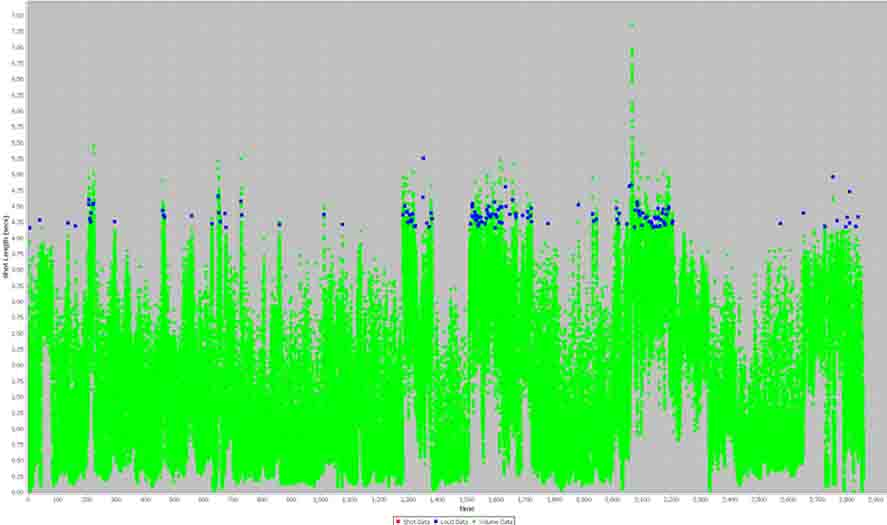
\includegraphics[trim = 0mm 0mm 0mm 0mm, clip, scale=0.35]{Images/doctor_who_loudness_graph.jpg}
\caption{Doctor Who Loudness Graph}
\end{center}
\end{figure}

\begin{figure}[h1]
\begin{center}
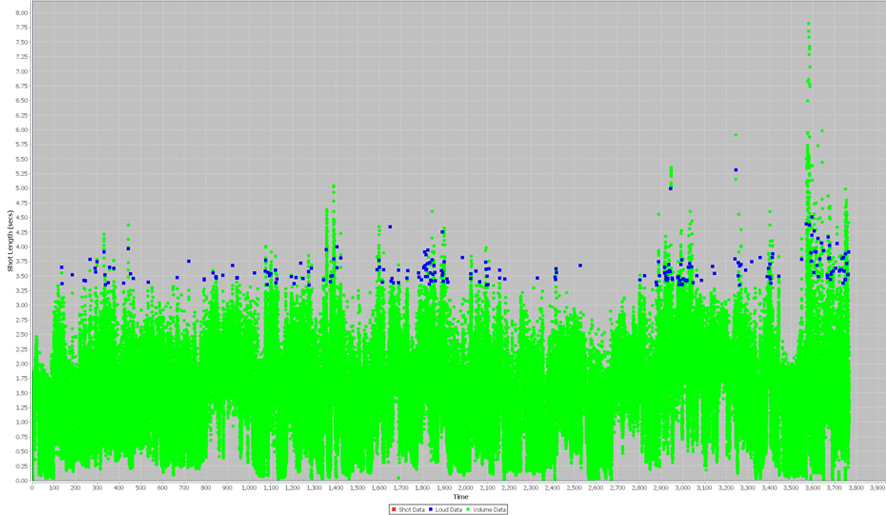
\includegraphics[trim = 0mm 0mm 0mm 0mm, clip, scale=0.35]{Images/top_gear_volume_graph.jpg}
\caption{Top Gear Loudness Graph}
\end{center}
\end{figure}

These graphs were compared to the volumes recorded by the team baring in mind the volumes recorded by the team was subjective and not too accurate due to human error. Areas noted as loud in our analysis matched the loud points plotted on the graph, likewise for quiet areas. However inaccuracies may be put down to the viewers inexperience.The volume detector performs as desired in detecting the loud sections and appears to be fairly accurate. 

In terms of speed, the volume detection process took 10 minutes to complete comparing this to manual inspection of the data which took approximatly 75 minutes. Therefore our process takes 13\% of the time to do it manually.

Volume detector functions correctly but unfortunately takes longer to process compared to other modules such as Name and Location Detection in Subtitles (see Section \ref{sec:Subtitles}), therefore an area of future work for this module would be to improve its module would be to improve its performance.

\newpage
\subsubsection{Face Recognition}
This element of the system remains unfinished as several problems still exist that the team did not have time to solve. Therefore this Section has been evaluated in terms of the different techniques used as opposed to its integration into the final product. 

\textbf{Facial Recognition Techniques:}
As detailed in the Facial Recognition Section (\ref{sec:FacialRecognition}) this section was broken down into three main components.

\begin{itemize}
	\item{Facial Detection}
	\item{Facial Clustering}
	\item{Facial Matching}
\end{itemize}

In order to evaluate the facial detection technique upon which the other two elements build, a minute of footage was gone through manually and the faces were identified. These results were then compared to those produced by the facial recognition code which uses the functions provided by the OpenImaj team \cite{citeOpenImaj}. \textbf{NB: These evaluations are being made purely on the final techniques as detailed in the facial recognition section and only the genuine faces are being judged as the aforementioned section looks at the issue of false positives}.

\underline{Manual Inspection of Facial Recognition}

\begin{center}
\begin{tabular}{|p{201pt}|p{201pt}|}
\hline
\textbf{Character Description} 	& \textbf{Total Appearances} 	\\\hline
Man in Wig			&25				\\\hline
Guard 1				&18					\\\hline
Guard 2				&18					\\\hline
Girl at painting			&10					\\\hline
Doctor				&7					\\\hline
Rory					&16					\\\hline
Amy					&16					\\\hline
\end{tabular}
\end{center}

\underline{Final Facial Detection Technique}
\begin{center}
\begin{tabular}{|p{160pt}|p{100pt}|p{134pt}|}
\hline
\textbf{Character Description} 	& \textbf{Total Appearances} 	&\textbf{Appearance Accuracy}	\\\hline
Man in Wig			&16					&(16/25) 64\%				\\\hline
Guard 1				&0					&(0/18) 0\%				\\\hline
Guard 2				&0					&(0/18) 0\%				\\\hline
Girl at painting			&0					&(0/10) 0\%				\\\hline
Doctor				&0					&(0/7) 0\%				\\\hline
Rory					&2					&(2/16) 13\%				\\\hline
Amy					&12					&(12/16) 75\%				\\\hline
\end{tabular}
\end{center}

The table above shows that some of the characters were very well identified and others were not. There are however understandable reasons for why both the guards and the doctor were not identified. The guards both appeared in the scene behind the man in the wig and were smaller and less clear to see. A similar issue occured with Rory and Amy as they both appeared in the same set of frames, although Rory did manage to log two detections. The doctor's head was the only visible part of him but he was at the bottom of the screen and rotated by about 90 degrees making him much harder to identify. Overall three of the characters were well identified and matched and those that appeared as sideline characters to a scene or weren't clearly displayed had less successful results. 

\underline{Final Facial Clustering Technique}
\begin{center}
\begin{tabular}{|p{160pt}|p{100pt}|p{134pt}|}
\hline
\textbf{Character Description} 	&\textbf{Faces Identified}					 	&\textbf{Cluster Accuracy}				\\\hline
Man in Wig			&10 in one set, 6 in another				&(10/16) 63\%					\\\hline
Rory					&2									&(2/2) 100\%					\\\hline
Amy					&11									&(11/12) 92\%					\\\hline
\end{tabular}
\end{center}

The table above shows the four characters that had their faces detected compared for clustering accuracy. Generally the clustering above produced good results with the images being clustered correctly with the only problems of the man in the wig being identified as two different characters, and some additional false positives that were matched with these faces. 

\underline{Final Facial Matching Technique}
\begin{center}
\begin{tabular}{|p{201pt}|p{201pt}|}
\hline
\textbf{Character Description} 	& \textbf{Actor Match Success }			\\\hline
Rory					&Not enough images to match	\\\hline
Amy					&Successfully Matched			\\\hline
\end{tabular}
\end{center}

The table above shows the two characters that were detected and had the potential for matches as both are main characters within the series. Karen Gillan was successfully matched with Amy Pond but Rory was unable to be matched as there were not enough instances of his face to train the recogniser. 

In conclusion to this, each element works well as far as building on the previous ones goes. However, it is difficult to determine how this would work running over a large set of videos as due to the memory problems of not being able to fully face detect a video this could not be tested further. However, each section has produced some successfull results and suggests that if the memory problems were solved and the issue of false positives was further tackled then these methods could be effectively combined to produce a significantly better facial recognition and detection system. Due to the problems this section was not encorporated into the summarisation element of the final product, however it can still be run individually through the system. 

\newpage
\subsubsection{Evaluating Video Shot Detection.}

Finding the breaks in video is a relatively straightforward thing for a person to do manually, but it is very time consuming, to do this accurately someone would have to watch the video back in normal time. If the user is only interested in counting the shots then a video can be processed at the speed the video is watched. However this only works for relatively short videos as the attention levels of the viewer have to be particularly high. 

If the viewer is interested in recording the time point of each start of shot, the record keeping is more difficult. Writing down a time point on paper would involve looking away from the video which means that the user is likely to miss the next shot.  This means the video will probably need to be paused periodically, depending on the video cut rate, this can easily make the time to find shots around double the length of the video.

In our system the shot detection for a 45 minute video, shot detection took 10 minutes 30 seconds. Our system shows a frame representing a particular shot in the GUI, it also presets the time that the shots appeared to the user. The shot time information is also then made available in the summary export and is plotted onto the graph. Again this would be a particularly time consuming task, and it’s speed of completion would depend on the skill of the viewer. This means that our application can complete the shot detection stage at around 8.5 times the speed of a human. This figure is likely to improve in our system’s favour as the length of video to process increases due to the high level of concentration needed to work through material.

The developers spent some time adjusting the sensitivity of the shot detector, this was done by watching a section of video and counting the shots, then allowing the system to do the same. We achieved a good level of accuracy and the system tended to differ on very fast camera movements, which occasionally happened in our Doctor Who test video. Some special effects such as flashes would also fool the system. This was not a particularly large issue for the system, due to the infrequency of errors. In addition, sequences of shots are combined as metrics are combined, and therefore the chances of impact on the final video summary are quite low. With more time to develop this area, additional testing could be done on different types of video. However as previously mentioned, manually finding and recording shots is too time consuming to do at any length in a project of this size and scope.

\subsubsection{Video Summary Evaluation}
Our system produces a video summary based on the various modules of our system. This
is based on:
\begin{itemize}
	\item{Person detection}
	\item{Location detection}
	\item{Loudness detection}
	\item{Shot detection}
\end{itemize}

As mentioned in Section \ref{sec:FacialRecognition} and \ref{sec:Music}, the team were not able to integrate the face detection and recognition or music detection at this stage, however the video summary output is a good representation of the loaded videos as demonstrated below.

\underline{Summary Shot Distribution}
\newline
Using three 45 min Doctor Who episodes, the team tested summary generation to check that a variety of shots from different episodes were included in the the video summary as well as checking that the duration parameter that the user sets restricts the maximum length of the video summary. The results of this testing are shown below:

\begin{itemize}
	\item{\textbf{Test 1:} Doctor Who (2005) Series 6 Episodes 1 - 3 (Episode length: 45 minutes).}
	\item{\textbf{Target time:} 10:00, actual 9:33.}
	\item{\textbf{Efficiency:} The time to summarise these videos was 16 minutes then a further 7 minutes to build the video summary. It takes less than a minute for someone to load in the videos and subtitles and perform a search of the open TV database. Therefore the total time is less than 24 minutes.}
\end{itemize}

Outlined in the table below is a comparison of manual and automated processing by the application for these episodes:

\begin{center}
\begin{tabular}{|p{150pt}|p{125pt}|p{125pt}|}
\hline
\textbf{Action (3 Episodes)}		&\textbf{Manual (minutes)}	&\textbf{AVSummariser}
\\\hline
Person Finding				&34 x 3 = 102		&0:05 x 3 = 0:15
\\\hline
Location Finding				&16 x 3 = 48		&0:05 x 3 = 0:15
\\\hline
Shot Detection (Recording times)	&45 x 3 = 135		&10:30 x 3 = 31:30
\\\hline
Loudness detection			&45 x 3 = 135		&10.00 x 3 = 30.00
\\\hline
total						&420				&Multicore machine total: 16min
\\\hline
\end{tabular}
\end{center}

The shot distribution for two summary lengths are displayed below and are ranked in interest order i.e. most important first.

10 minute summary:
\begin{itemize}
	\item{Episode 1}
	\item{Episode 1}
	\item{Episode 1}
	\item{Episode 1}
	\item{Episode 3}
	\item{Episode 1}
	\item{Episode 1}
	\item{Episode 1}
\end{itemize}

15 minute summary:
\begin{itemize}
	\item{Episode 1}
	\item{Episode 2}
	\item{Episode 1}
	\item{Episode 1}
	\item{Episode 1}
	\item{Episode 3}
	\item{Episode 3}
	\item{Episode 1}
	\item{Episode 2}
	\item{Episode 1}
	\item{Episode 1}
	\item{Episode 1}
\end{itemize}

As can be seen from the two tests above, the interesting points of the three Doctor Who
episodes tend to fall in episode one as this is the introduction to the series with many major events. However, the system clearly uses shots from all episodes and produces summaries that are either equal to or slightly less than the target length in all tests.

\subsubsection{Video Summary Content Analysis}
The video summary produced has also been evaluated to check that the most important points in a episode have been included. The television programmes which have been used are as follows:

\begin{itemize}
	\item{Top Gear Series 9 Episode 3 - US Special}
	\item{Top Gear Series 14 Episode 6 - Bolivia Special}
	\item{Doctor Who (2005) Series 2 Episode 12 - Army of Ghosts}
	\item{Doctor Who (2005) Series 2 Episode 13 - Doomsday}
\end{itemize}

Appendix \ref{sec:TV} contains the manual inspection of these episodes as well as the comparison of which points made it into the summary. Each test has been done by viewing each episode and documenting the interesting features. Using this data the output video summary could be watched and compared with the results noted alongside the original observations. Note this was done using the default trailer type.

Limitations of this approach are that it is subjective about what are the important points in an episode. This is a difficult problem to avoid which is why the team used a number of different videos however to improve test results this process could be done on varying television programmes and using a greater number of test subjects. But due to the time restriction of this project this wasn’t possible.

As a whole the system picks up a good number of important points; the breakdown per episode is below:

\begin{center}
\begin{table}[ht]
\begin{tabular}{|p{150pt}|p{90pt}|p{90pt}|p{50pt}|}
\hline
\textbf{Episode}	&\textbf{No. of Interesting Points}	&\textbf{No. of matches in Summary}	&\textbf{Percentage}
\\\hline
Top Gear Series 9 Episode 3 - US Special&17	&2	&12\% \\\hline
Top Gear Series 14 Episode 6 - Bolivia Special&14	&3	&21\% \\\hline
Doctor Who (2005) Series 2 Episode 12 - Army of Ghosts&24	&6	&25 \\\hline
Doctor Who (2005) Series 2 Episode 13 - Doomsday	&8	&2	&25\% \\\hline
\end{tabular}
\caption{Interest Point Matches}
\end{table}
\end{center}

On average 21\% of important points are identified which demonstrates that the system at this time didn’t perform well for this experiment, which may be due to the particular trailer type being used or the team’s opinion of the most interesting points. Therefore further testing is needed and there are areas which can be improved to increase the identification percentage are detailed in Section ref{sec:FutureWork}.  For example r- running the test on Top Gear Series 9 Episode 3 - US Special using the People mentioned trailer type, it produced a 24\% match rate.

There are output videos which the system has produced in Appendix \ref{sec:CD} are available on the CD.

\subsubsection{Non-Functional Evaluation}
The first non-functional requirement (NF1) was that the new system should be able to handle the BBC’s file formats available from their research archive. The team encountered an issue at the video concatenation stage with the “.ts” file format. This was worked around by using the unix ffmpeg utility to convert the video to mp4. This is a commonly used utility which the software depends on through the Xuggle library so this was not judged to be a major issue by the team. 

The software accomplishes the objective to export the data in a standard format. (NF2)The data is output in XML format and the video in MP4. This is compatible with all popular operating systems. The application has a status bar at the bottom of the GUI, which informs the user of progress at the various stages, most importantly through summarising stages which can take a significant period of time. 
The third requirement NF3: processing the broadcast data faster than a user could watch the video. This point has been covered in the other evaluation sections. The application is relatively efficient as it is multi-threaded (NF5), and the team recognised the significant impact that this had on performance. The application that the team have produced processes videos with separate threads for the various modules, this means that the application runs much faster on a modern machine with multiple cores than something that is a few years old. Finally, as already mentioned earlier in the project we have built the system upon the OpenIMAJ library. 

\newpage
\subsection{Evaluation of the Team Dynamics}
\label{sec:EvaluationTeam}

The team was formed the previous semester (Spring semester 2011) through shared
friendships and the belief that each individual would work well with the
others. The teams previous history working together through solo and group
courseworks allowed each team member to know the strengths and weaknesses of the
others before the project began. Such prior knowledge allowed the team to
allocate job roles based upon their previous experience with one another as
shown in \ref{tab:TeamRoles}. These job roles though quite vague, did prove to
match each individuals tasks throughout the project.

To ensure the team never had serious discontent between team members
it was decided at the offset of the project to have regular meetings within the team
where issues could be aired and problems vented within the team throughout the
week to ensure they would not become serious issues between team members. As
shown in Section \ref{sec:TeamMeetings} the team met each Monday and Friday in a
formal manner to discuss issues that had arisen over the weekend and during the
course of the week. Such regular meetings meant that there were no issues
between team members that were not resolved swiftly.

In addition to regular meetings, communication between these meeting times was
also decided to be vital to the team. As may be seen in Section
\ref{sec:communicationAids} the team had decided upon always being contactable
through a number of methods, dependent upon time of day and their location. Each
team member shared with the others their contact details and throughout the
project each team member was capable of contacting the others through one or the
other of the prescribed means with a generally swift response. A more concrete
agreement about what means to contact each other through may have made the team
more effective since different individuals often contacted one another through
different mediums dependent upon their preferences so it was found that quite a
few software tools and pieces of hardware had to be checked often to ensure that
no communication from other team members was missed. Google chat was also under
utilised as an instant messenger (IM) form of communication since it is a
browser based form of IM. A better form of IM may have been hotmail or skype
with a seperate piece of software which logs the user in when they connect to
the web without their assistance since often members would be online, but not
signed into Google talk.

The final core part of the team dynamics was pair programming. As with the
others pair programming was a planned part of the team's works from the onset of
the project, as shown in Section \ref{PairProgramming} which coupled with peer
review (Section \ref{PeerReview}) was intended to create a shared knowledge base
of the projects source code. Pair programming was under utilised the teams
believes, though some pair programming was engaged upon not as much as was
planned for was completed. Unfortunately what the team was trying to prevent
from occuring did happen, where only one individual has knowledge of a section
of code. Such specialisms did occur throughout the project often causing team
members to be unsure of one anothers work and what was present else where in the
code. Fortunately through the frequent meetings and communication channels these
specialisms were not allowed to become an issue, but the coding of the project
could have been better managed.

\newpage
\subsection{Evaluation of the Project Management}

The planning and management of the project was all decided upon during the
inital two weeks of the project. During these two initial weeks the team chose
methods of development and planned their projected tasks for the whole project.
In Section \ref{sec:ProjectManagement} and Section \ref{sec:SoftwareModel}the
team details their decisions upon the tools to use for project management and
the method they chose for their software model, which was the iterative
waterfall model. The chose of software model directly effects the ways in which
the team is managed. For instance an agile method such as Scrums would result in
a more individualistic approach to team management within a scrum, but then a
team based approach to time management at the start of each scrum. The choice of
the iterative waterfall model meant for the team that it was only once a task
was completed was it possible to be reviewed and then potentially worked
further upon as was deemed necessary. Such a model meant that the projects
management was often not aware of the all the team members status upon their
various tasks until the time for completion was reached, at which point their
states were reviewed and often extended. That meant often problems with a task
would not become visable to the team until it was at the point of becoming a
problem. Preferably a model where team members were constantly updated of one
anothers progress would have been used so that others could have become involved
with one anothers work as assistance before the tasks became a team wide issue.
As discussed in Section \ref{sec:EvaluationTeam} the team did not complete as
many tasks as desired using pair programming which exacerbated the issue of team
members being unaware of one anothers current states.

Team management breakdown into two more specific areas, time management and
resource management. The following sections evaluate how well these were done
within the team.

\subsubsection{Time Management}
\label{sec:timeManagementEval}
This section details how well the team progressed during this project and how effectively we managed our time and whether we achieved our project milestones. This evaluation will be done by comparing the initial gantt chart we produced at the beginning of the project and the current version; these are shown in Appendix \ref{sec:GanttChart}.

A table below compares the start and end time of each of our project stages:
\begin{center}
\begin{tabular}{|l|l|l|}
\hline
\textbf{Stage}					&\textbf{Initial Gantt Chart}		&\textbf{Final Gantt Chart}	\\\hline
Planning					&					&				\\\hline
\hspace{5mm}Started		&3/10/11			&3/10/11		\\\hline
\hspace{5mm}Completed	&14/10/11			&19/10/11		\\\hline
Design					&					&				\\\hline
\hspace{5mm}Started		&5/10/11			&5/10/11		\\\hline
\hspace{5mm}Completed	&19/10/11			&21/10/11		\\\hline
Implementation			&					&				\\\hline
\hspace{5mm}Started		&14/10/11			&14/10/11		\\\hline
\hspace{5mm}Completed	&18/11/11			&8/12/11		\\\hline
Verification				&					&				\\\hline
\hspace{5mm}Started		&19/10/11			&16/10/11		\\\hline
\hspace{5mm}Completed	&25/11/11			&13/12/11		\\\hline
\end{tabular}
\end{center}

As shown in the table above the project schedule changed significantly between the initial and current gantt charts; the reasons why the project progress got delayed is discussed below. 

Firstly, is that the team found particular tasks in this project difficult which is due to the lack of experience and knowledge the team has in this area, as identified in the risk analysis (see Section \label{sec:Risks}). Leading on from this point, the team underestimated the enormity of the tasks involved with this project in the Planning stage which is one of the reasons why some of the tasks discussed in this report are incomplete such as Face Detection and Music Detection.

Another reason is that the OpenIMAJ library \cite{citeOpenImaj} which the team used as part of the Implementation stage of the project was in development during the project and was presented at the ACM Multimedia 2011 \cite{competition} this led to the team having to overcome bugs and issues that were found whilst implementing and creating workarounds which then had to be re written once these issues were solved. Despite these problems, the library helped in completing the tasks involved within this project which the team probably wouldn't have completed without their help due to the team’s lack of experience in this area as mentioned.

Thirdly, the team have had to deal with other module coursework clashes in particular COMP6017 Web Services which three members of this team are undertaking. Due to the difficulty and effort that was required for this piece of work, a team member had to allocate all their time to that coursework in order that it could be completed on time despite those team members working on this coursework from when it was received and balancing their time between this and that coursework. Therefore their work was rebalanced among the rest of the team members in order to keep progressing.

Finally, as the system was implemented and the different modules were integrated together it became apparent that the team’s development environments were not suitable in terms of processing power and struggled in running all the integrated modules together to produce the final summary. Although this have an impact in the project progress as much as the other reasons stated.

In conclusion, the team has worked effectively to overcome these challenges in terms of planning ahead, re balancing work as necessary and communicating with the OpenIMAJ development team to solve any technical issues the team had during the Implementation stage of this project.

\subsubsection{Resource Management}

The sole real resource other than time that the team's project had were the team
members themselves. As previously discussed in Section \ref{sec:TeamStrengths}
each team member has their own personal strengths and weaknesses thus managing
those tasks which team member, or recourse is deployed upon is critical to
ensure effective management of these resources. For instance a resource which is
designated the lead programmer through their strong programming experience
should not be deployed upon documentation tasks when there are other programming
tasks which they could be utilised more effectively on.

Such resource management was performed fairly effectively through selfelective
task choosing from the team members. Each team member chose from the upcoming
tasks those tasks which they felt they would be best at. Such selfselection of
tasks did result in fairly effective resource deployment though occasionally
larger or more challenging tasks were left to whoever was willing to or was
voted suited for task to pick up rather than chosen by a team member. 

A more effective method of resource management would be preferable in the
future, but without a manager who knows the capabilities of each team members as
intimately as themselves the balance between what a resource can achieve well
and what they enjoy would not be reached. As far as the team is aware no more
effective and fair method could be found than the one they used, but as shown it
did have its failings.